%%% Made of Tiny Robots
%%% An Investigation of the Ecology of Responsive Environments
%%%
\chapter{An Ontology of Responsive Environments}
\label{ch:ontology}
%
As we enter the age of ubiquitous computing our relationship with our artifact ecology is changing. 
There are several factors to these changes: we have new ways to fabricate artifacts; we have new ways of relating to artifacts; and our artifacts increasingly perform tasks that were once the exclusive domain of people.

To help to understand these changes we first develop a vision of the means of production within a responsive environment (in Section~\ref{sec:production}) and the roles that people can play in producing and interacting with responsive artifacts (in Section~\ref{sec:roles}). In Section~\ref{sec:artifact_ecologies} we then describe how people adopting these different roles interact within the artifact ecologies introduced in Chapter~\ref{ch:intro}. 
We suggest that one of the key distinctions between these different ecologies is the roles that are available for members of each society to play; ecologies structured around more transparent technological mechanisms and more reconfigurable artifacts will present more opportunities for people to adopt roles that shape the behavior of their environment. 
Of particular interest is what we are calling a robunculi ecology: manufacturing is focused on producing robotic kits of parts rather than devices that perform a single role; these kits can either be assembled, or can self-assemble, into a variety of forms on demand.

After describing this ecological backdrop, in the following sections we delve into the range of characteristics potentially exhibited by responsive artifacts themselves. In Section~\ref{sec:purposes} we characterize several categories of purposes for which responsive artifacts could be intended. In Section~\ref{sec:morphologies} we discuss manipulative and other morphologies. We describe the pairs of synergistic input/output affordances that characterize responsive artifacts in Section~\ref{sec:affordances}. We describe several \emph{devotions}, modes of data collection that artifacts can perform in service of idols, in Section~\ref{sec:devotions}. And in Section~\ref{sec:characterizing} we collect together the five categories of features of responsive artifacts we have introduced with a set of icons that we will apply in the following chapters to characterize individual projects.

\section{Artifact Production}
\label{sec:production}
%
In a popsicle ecology we are used to purchasing packaged preconfigured devices. As illustrated in Figure~\ref{fig:hardware_venn} there are several ways a device can be implemented in a responsive environment. 

\begin{figure}[b!]
  \centering
    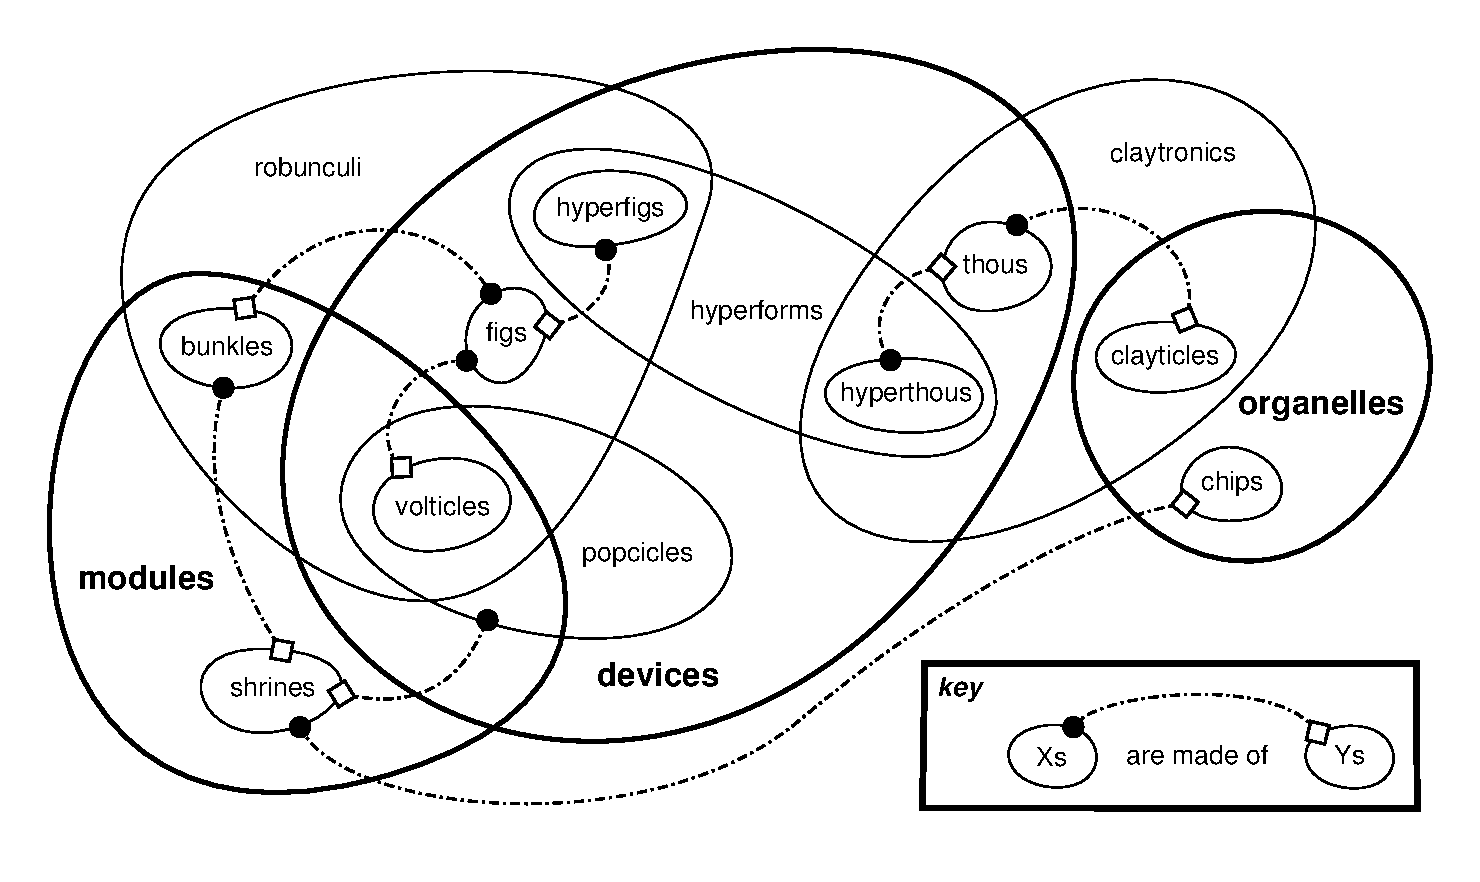
\includegraphics[width=140mm]{hardware_venn.pdf}
  \caption{Venn diagram of computational artifact hardware categories.}
  \label{fig:hardware_venn}
\end{figure}

Two important factors in the production of responsive hardware are scale and tooling. 
At the smallest end are chips, analog electronic components, sensors and actuators. 
We will refer to this group collectively as \emph{organelles}, after the tiny machines that power biological cells; these components are generally produced in high volumes in and require expensive, technologically sophisticated tooling usually found in factories. 
Even supposedly \textbf{open hardware} systems are built around these closed organelles. 

At the next scale are modules that package these organelles to make them more accessible to spoke developers (for example an Arduino board), or to present a tangible interface (like our Posey kit). 
(The Arduino is an example of a \emph{shrine}, a computing module that can, among other things, allow a device to communicate with idols.) 
This stage of production can take place at a sophisticated local fab shop (with tools such as a \textbf{pick-and-place}) but often takes place in a more traditional factory because of the economic advantages of scale.

Popsicles are generally manufactured as a monolithic design including the necessary organelles on a custom circuit board, and sandwiched inside of a factory-produced case. 
Spoke and robunculi ecologies make use of modules to lower the barrier to device design. 
Sharing high-level components reduces the amount of technological knowledge required to create and customize devices.
Open hardware circuit modules abstract away from the complexity of organelles and electronics, and are generally accompanied by online code samples and tutorials. 
Open hardware designs for cases and mechanical components can also be downloaded, customized and then fabricated with \textbf{rapid prototyping}%
\footnote{Some examples of rapid prototyping technologies commonly available at local fab shops are \textbf{fused deposition modeling (FDM)} \textbf{3D printers} and \textbf{computer numerically controlled (CNC) mills}.}
technologies at local fab shops (such as \textbf{hackerspaces}).
Producing a device with robunculi requires no manufacturing at all, a device can be realized by assembling it from bunkles, or by loading a program so that it self-reconfigures.

With robunculi systems the artifacts being manufactured are no longer devices but rather kits of \emph{bunkles} (our term for an individual robunculi module; analogous to a single lego brick) that can be used to create devices (among other things). We call a device that is implemented as a particular configuration of bunkles a \emph{fig} (as in a configuration). Robunculi make customization of a device design as accessible as playing with a construction kit. They support reuse by allowing different figs to be implemented at different times with the same bunkles. And a kit can be customized by printing new bespoke bunkles at a local fab shop.

While a single bunkle is not generally useful without a whole kit, it is possible that a device such as crystal (i.e. a smart phone) could interoperate with robunculi;%
\footnote{For example Google and Arduino collaborated to produce the Arduino Mega Android Development Kit (\url{http://labs.arduino.cc/ADK/Index}), an open hardware module for creating spokes that interface with devices running the Android operating system.}
it could be connected as a part of a fig to provide a display, or better networking, or a more powerful processor.
We will call such a device that can function both on its own (as a popsicle) and as a part of a fig a \emph{volticle}, an abbreviation of `Voltron%
\footnote{Voltron is a fictional \textbf{mecha} from the Japanese animated series of the same name. It is composed of five smaller mechas that can operate on their own or join together to form Voltron.}
popsicle'.
Volticles are one example of how spoke and robunculi ecologies can influence larger popsicle ecologies to support transparency and reconfiguration.

Robunculi capable of self-reconfiguration can be used to create hyperforms (objects capable of changing their shape over time). We call a robunculi hyperform a \emph{hyperfig}; one useful way of characterizing a hyperfig is by defining a series of intermediate fig keyframes that the system self-reconfigures between. 

Hyperforms can also be implemented by claytronic systems. While robunculi are composed of bunkle modules claytronic systems are composed of tiny clayticle organelles. We call the claytronic analog of a fig a \emph{thou} after the T-1000, the shape-changing robot made of `liquid metal' from the 1991 movie Terminator 2. A self-reconfiguring claytronic system could be used to implement \emph{hyperthous}. In the example of the T-1000 (Figure~\ref{fig:t1000_weapon_thou}), it is capable of assuming a thou that mimics an actual person. Its hyperthou involves rapid self-reconfiguration of just the limbs of these mimic thous into piercing or slashing weaponized thous, as befits a killer robot from the future. 

\begin{figure}[]
  \centering
    
\includegraphics[width=80mm]{t1000_weapon_thou.jpg}
  \caption{Still from \emph{Terminator 2} showing the T-1000 implementing a mimic thou with a weapon thou in place of its left arm.}
  \label{fig:t1000_weapon_thou}
\end{figure}



\section{Roles for Responsive Environments}
\label{sec:roles}
%
One of the most important aspects of an artifact ecology are the roles available for people to relate to the artifacts within it. In some ecologies only a select few highly trained professionals have any input on the behavior of devices, while other ecologies provide opportunities for a broader spectrum of society to participate. We will not discuss the role a `user' of a locked-down device plays, but only roles that allow some level of input back into the larger ecology.

The roles described here are not meant to define individual people, but rather are different stances that a single person could take toward an artifact at different times. For example a researcher that designs prismatic cube bunkles could also take on the role of a fig designer and create a social table hyperfig. And then later at home the same person could eat dinner at a social table and write up an evaluation of the experience.

The roles are also not separated by discipline (e.g. electrical, mechanical, code) but by level of accessibility. This reflects the ideal of open hardware design that a single person can have an idea for a device and build a prototype to demonstrate it. Spoke and robunculi ecologies attempt to support this development model by packaging the more technologically demanding features in reusable modules. And our organization of roles reflects the reality that modules often span these disciplinary boundaries. (For example the Arduino project packages both electrical and software components, and many of its extension modules include mechanical, electrical and software bits.)

\subsection{Taster}
A person adopting this role, for example a person sitting down at a social table, is relatively passive in relation to the artifact in question. Tasters participate in the ecology by providing critical feedback in relevant forums. This could be as simple as having a specialized gesture expressing approval (or disapproval) of a given hyperfig that is then incorporated into rankings on the online hyperfig repository, or as involved as filing a bug report.

While even in a popsicle ecology journalists and bloggers can play this role, the online design repositories of spoke and robunculi ecologies provide an opportunity for tasters' feedback to be used as debugging data and a filter for identifying successful systems. 

\subsection{Wrangler}
Many devices require substantial input from a person, for example many military sockpuppet drones are operated remotely by a trained pilot at a stickboard. While adopting the roles described below requires some kind of expertise in customizing or building devices, wrangling demands expertise at piloting or otherwise managing devices' behavior in real time.

As wranglers possess a unique perpsective on the behavior of the devices they wrangle, it would be desirable for ecologies to also attract wranglers to serve in design roles. Tinker roles in particular (discussed below) offer an opportunity for wranglers to give design input without a great deal of investment in training.

\subsection{Tinker}
Many people are motivated to understand more about the mechanisms underlying the behavior of responsive devices but lack the technical knowledge required to address systems at the same level as their designers. 
A strategy for engaging this community is to create devices with tink interfaces. 
An example is a golem robunculi with instructions for building a given golem that can then be varied, much like lego kits come with instructions that can serve as a jumping-off point for more creative endeavors. 
And while such mechanical tinkering is straightforward, tangible interfaces can also be used to allow tinkering with algorithms%
\footnote{For example Scratch \citep{scratch} has established a model for a visual, fault tolerant tinkering-style programming interface that involves shuffling puzzle-piece chunks of code, although it is screen-based. 
Tern \citep{tern_classroom} applies similar ideas with a tangible interface composed of literal wooden puzzle pieces. 
With Cubelets (nee RoBlocks) \citep{roblocks} a fig specifies both mechanical and algorithmic properties at once.} 
and electronics%
\footnote{For example littleBits \citep{littlebits} package electronic components to afford tinkering with circuits.}.

By providing opportunities for people to tinker with their devices robunculi ecologies can help to both engage people in a conversation about their devices, and recruit people to expand their technological capabilites so that they are able to adopt more technologically demanding roles. By providing places for people to expand and apply their skills, a spoke ecology and its associated hackerspaces can help these new recruits find productive technical roles to play.

\subsection{Tek}
Here we have reached the realm of the professional designer (and engineer). A tek is a person who comes up with ideas for and builds new devices. 
While professional designers are traditionally grouped according to their specialized technical discipline, we suggest that such compartmentalization works against a tek's ability to envision and create useful devices. 

In particular, within spoke and robunculi ecologies the availability of modules that package complex technologies lower the barrier to assuming the role of a tek. 
With robunculi the distinction between a tinker and a tek is even somewhat blurred, but as we will describe in Chapter~\ref{ch:case_studies} the creation of a device with new behaviors (rather than a variation on an existing device) will generally involve more advanced tools alongside the bunkles themselves, requiring tek-level proficiency.
We predict that the character of these artifact ecologies with a broad community of people able to assume the role of device designers will contrast sharply with popsicle-dominated ecologies where the character and behavior of devices are largely dictated to the community.

\subsection{Tooler}
Much of the growth of the open hardware scene and the spoke ecology comes from people who are thinking not about creating devices, but about the tools that can help teks to create devices. In doing so these people are assuming the role of a tooler. While a tooler may build a literal tool, such as a 3D printer, they also focus on packaging technologies in modules that make them more accessible. This is common practice in software development (even in popsicle ecologies) and is quickly spreading to electronic and mechanical development in spoke and robunculi ecologies. Again, toolers are not generally defined by discipline as many modules package components from several disciplines. In robunculi ecologies toolers design the bunkles (and their control algorithms) that teks and tinkers use to create devices.

\subsection{Wiz}
Because of the complexity of the technologies involved in creating responsive artifacts, at some point there is a demand for specialization. 
We call someone who considers the deep issues of a discipline, either to extend what can be done, or to make its capabilities more accessible, a wiz.
In adopting the role of a wiz a person could be developing a new programming language, designing a computer chip, developing a new actuator, or creating a new rapid fabrication technology. 
While people able to play such a role are generally prized in any artifact ecology, we suggest that expanding the community of teks has the potential to develop a greater number of wizs, thus advancing the capabilities of the entire ecology.

\section{Production and Roles in Artifact Ecologies}
\label{sec:artifact_ecologies}
%
In Chapter~\ref{ch:intro} we characterized several emerging ecologies in which responsive artifacts can be produced and deployed. We suggested that these ecologies differ significantly in the level of control average citizens have over the behavior of the artifacts in their environment. Here we detail the roles available to people within these ecological niches and discuss the effect these differences have on empowering people to participate in specifying the behavior of their robotic companions (or not).

We illustrate the relations of production and roles in these ecologies with some diagrams. These diagrams focus on entities that make a meaningful contribution to specifying the behavior of artifacts, and the roles people adopt in doing so. These diagrams present a relatively crude picture of complex phenomena, but even so serve to illustrate some striking differences.

\subsection{Popsicle Ecologies}
%
\begin{figure}[b!]
  \centering
    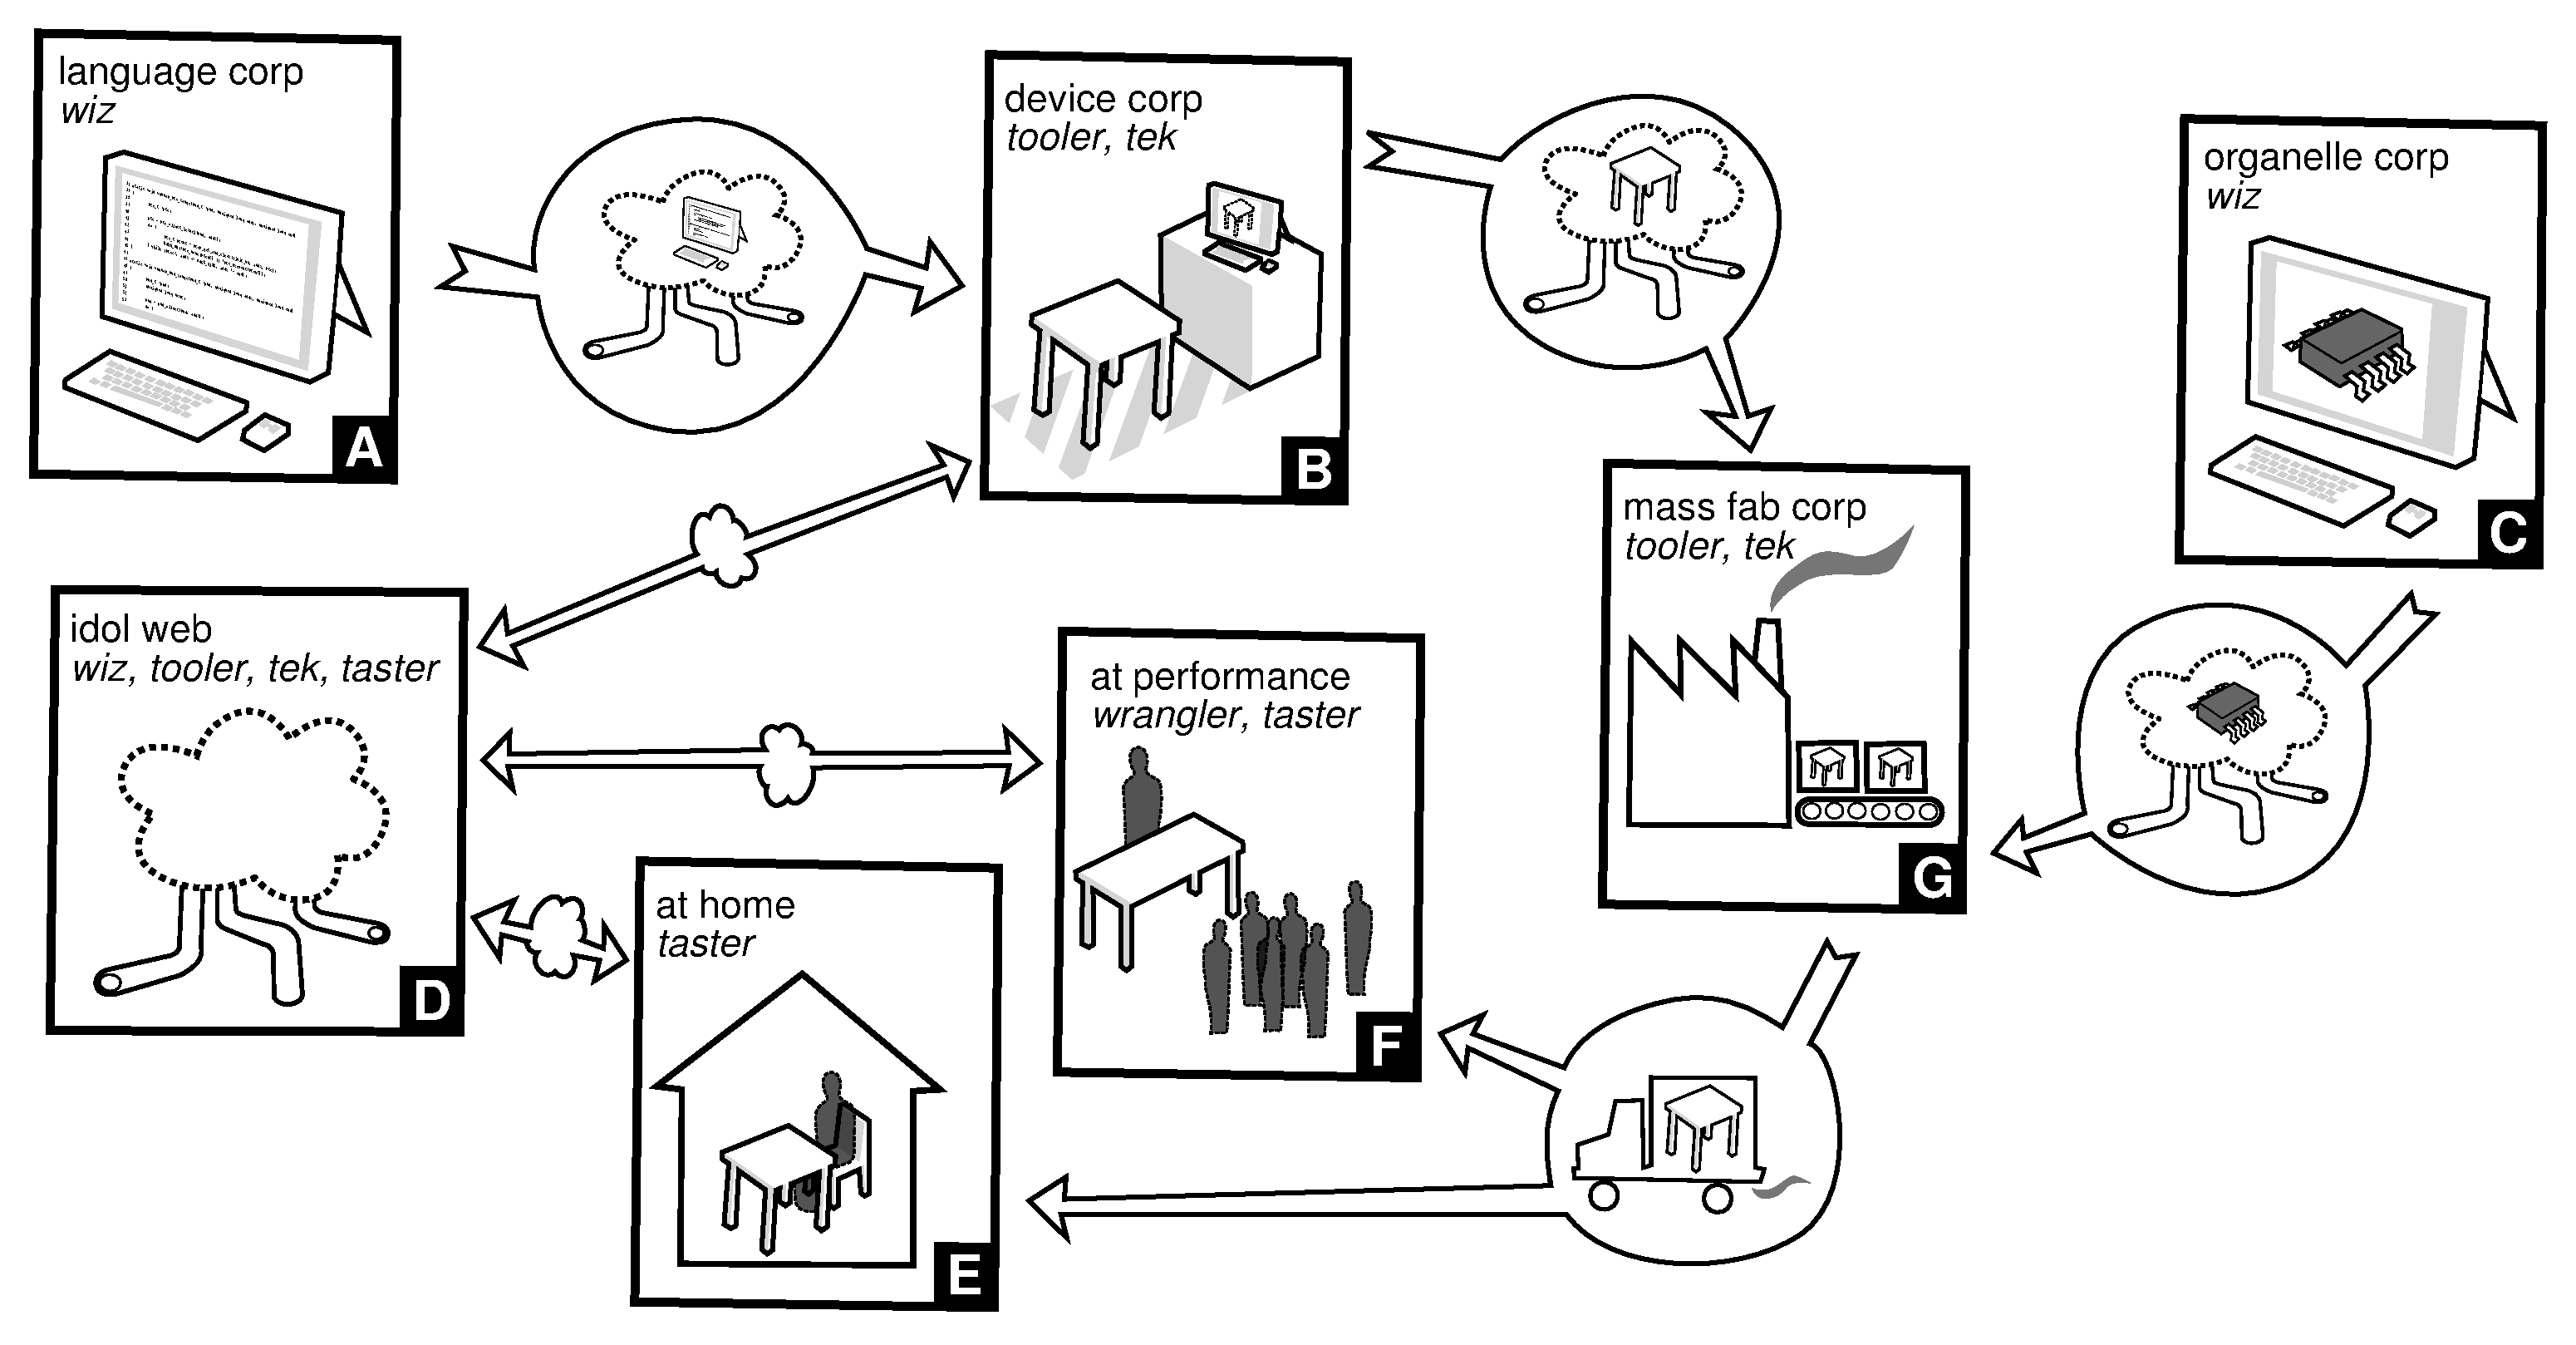
\includegraphics[width=130mm]{popsicle_ecology.pdf}
  \caption{Production and roles within a popsicle ecology.}
  \label{fig:popsicle_ecology}
\end{figure}
%
This ecology is the simplest---there are relatively few people involved in creating artifacts, and relatively few roles available for non-professionals to adopt in relation to their artifacts.
Figure~\ref{fig:popsicle_ecology} depicts the development of a hypothetical popsicle, a table with a crystal embedded in the surface.
The hardware is developed internally by a single company (Figure~\ref{fig:popsicle_ecology} at \emph{B}). The design leverages a few reusable packages developed internally by the company's toolers, but is largely developed by company teks drawing on previous design iterations. The device is built around  a \textbf{system on chip (SoC)} organelle%
\footnote{An example is Qualcomm's Snapdragon that handles processing, graphics, and both cellular and wifi networking for crystals.}
developed by circuit wizzes employed at an organelle corporation (\emph{C}).
This hardware is then combined with an operating system developed for tabletop crystals by language wizzes at a software company (\emph{A}).%
\footnote{Another device company developed the software for its competing iTable internally.} 
Both the device and its organelles are produced and assembled (and loaded with software) by toolers and teks at specialized manufacturers (\emph{G}) that operate enormous factories. 
The high cost of the specialized buildings and tools (especially for producing organelles) is amortized over the large number of devices produced.

Several versions of this table crystal are produced, including a professional model for electronic musicians and another version marketed for home use. The professional version is used by wranglers to perform shows (\emph{F}) for a group of tasters. The other version is used by tasters at home (\emph{E}). In this ecology wranglers and tasters have no direct input on the behavior of their table crystals, but can post their opinion on blogs or online forums (\emph{D}). Teks and toolers at the device companies can follow these posts with the assistance of idols and can potentially consider this input.

\subsection{Spoke Ecologies}
%
\begin{figure}[b!]
  \centering
    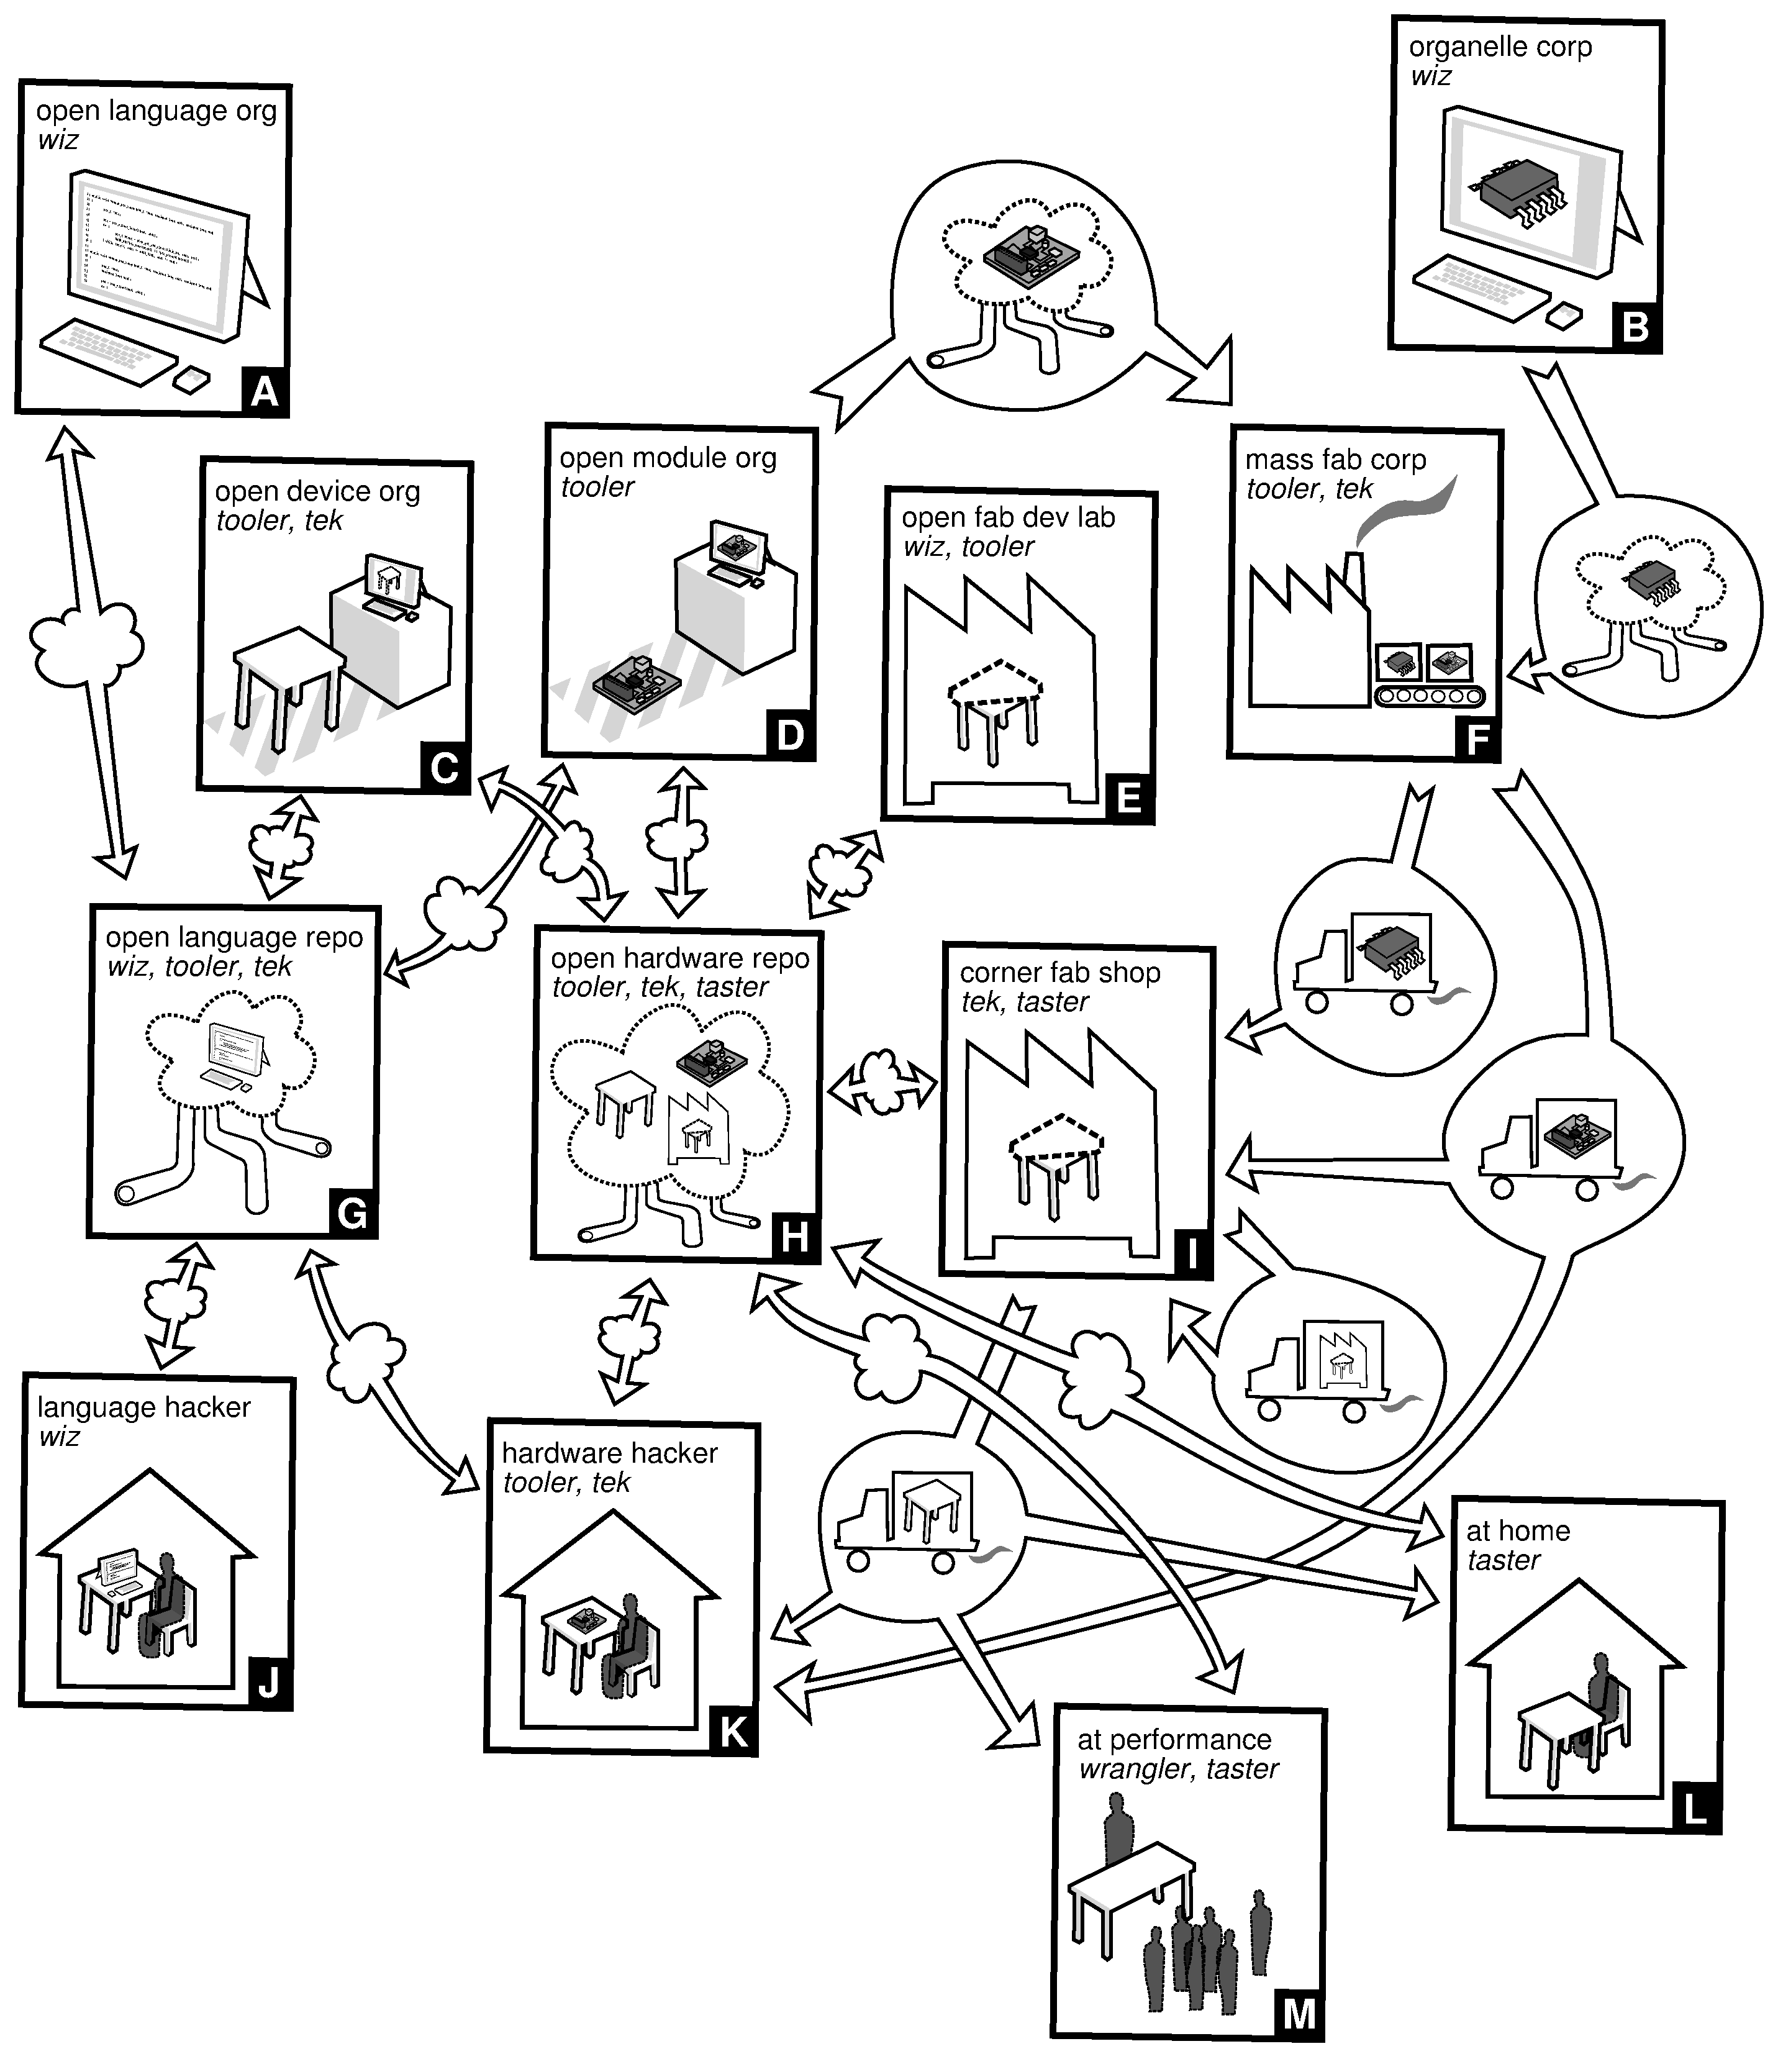
\includegraphics[width=130mm]{spoke_ecology.pdf}
  \caption{Production and roles within a spoke ecology.}
  \label{fig:spoke_ecology}
\end{figure}
%
With spoke ecologies  (Figure~\ref{fig:spoke_ecology}) we see the emergence of online repositories---for both code (\emph{G}) and hardware specs (\emph{H})---as a means of coordinating a distributed, open design process. The wizzes of open code development organizations engage with a community of volunteer language hacker wizzes (\emph{J}) as well as the toolers and teks making use of their code (\emph{C}, \emph{D} and \emph{K}).

These ecologies are defined by a shift from devices produced by large manufacturers (\emph{F}) to custom built devices assembled in neighborhood fabs (\emph{I}). 
Large manufacturers still produce organelles, which are still designed by wizzes at organelle companies (\emph{B}). Organelles are packaged in open hardware modules (such as the Arduino). 
Many parties may contribute to a design from academic labs%
\footnote{Such as New York University's Interactive Telecommunications Program  and the now defunct Interaction Design Institute Ivrea that incubated the Arduino project.}
to online retailers%
\footnote{Such as Adafruit, Sparkfun and Seeed Studio.},
to individual device hackers.
By coordinating through online hardware repositories (\emph{H}) these parties may contribute original designs, modify existing designs, manufacture modules, or all three.

The facilities for combining open software and open hardware modules to create a spoke are provided at local fab shops (\emph{I}).
These facilities feature rapid prototyping tools, many of which are themselves open hardware designs developed at academic research labs (\emph{E}) and produced at other local fab shops.
Teks employed at these shops can provide advice and assistance on spoke projects for those with the technical know-how to produce their own designs, or can produce custom works on commission. 
These custom designs can then be posted back to an open hardware repo to continue the design conversation, either by the local fab shop (\emph{I}) or the tasters and wranglers using them (\emph{L} and \emph{M}).

As in a popsicle ecology, many of the parties in this scenario post on blogs and forums. We left that activity off of this diagram as all parties have more direct means of contributing to the design process. Of course, fewer people are able to participate in this ecology as to produce a spoke one must be able to either adopt the role of a tek or have the resources to commission a tek to produce it. Although these ecologies may not produce as many devices as a popsicle ecology, they help to teach more people the skills to contribute to the design space. This can in turn effect popsicle ecologies---for example there are several open source operating systems for popsicle crystals (distributed in a similar manner to spoke software) that motivated people can load onto their devices to customize their behavior.

\subsection{Robunculi Ecologies}
%
\begin{figure}[b!]
  \centering
    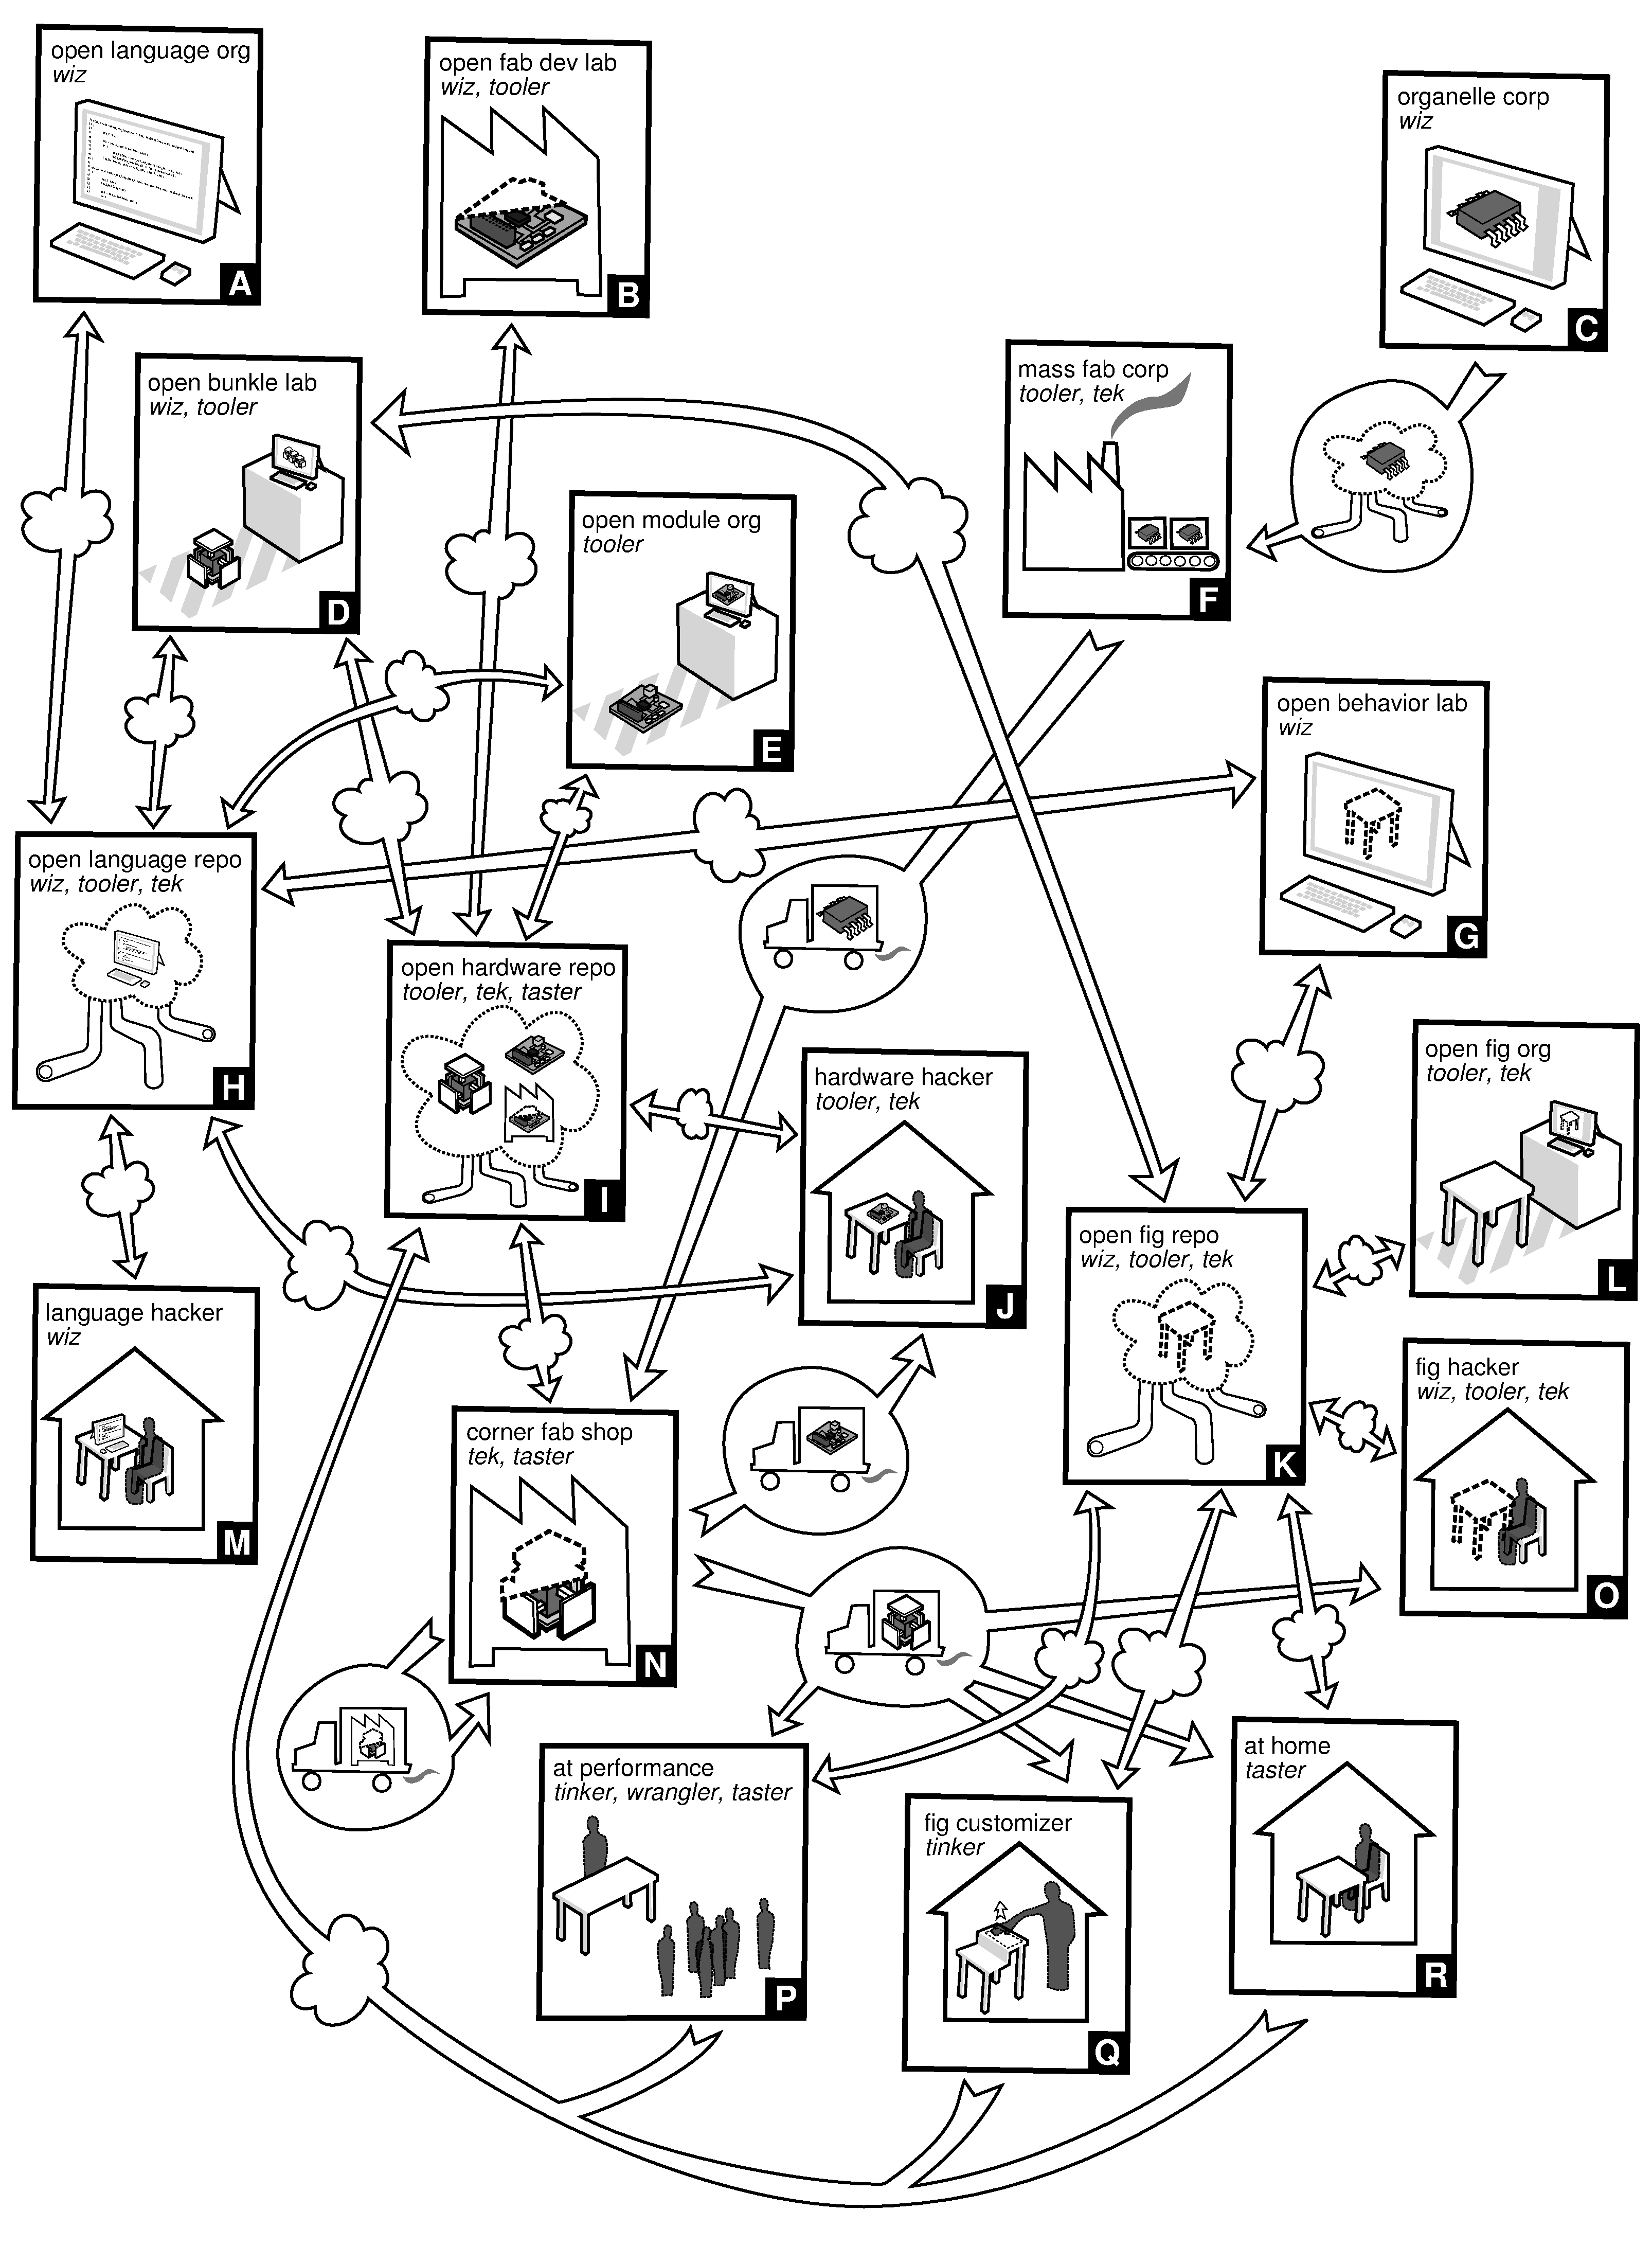
\includegraphics[width=\textwidth]{robunculi_ecology.pdf}
  \caption{Production and roles within a robunculi ecology.}
  \label{fig:robunculi_ecology}
\end{figure}
%
To simplify this already complex scenario---illustrated in Figure~\ref{fig:robunculi_ecology}---we are supposing that corner fab shops (\emph{I}) have advanced open hardware fabricators (developed by open fabricator development labs at \emph{E}) capable of printing out circuits and structural components.
By feeding in the appropriate organelles and feedstock such a machine could print a functional bunkle with little or no manual assembly required.
As a result relatively large numbers of bunkles can be produced on demand in local fabs and only organelles are still produced in large factories (\emph{F}).

Our diagram of this technologically advanced robunculi ecology is still the most complex as there are so many roles capable of making contributions. 
As in a spoke ecology there are online repositories for managing code (\emph{H}) and hardware specifications (\emph{I}).
There is also a new class of repository for fig specifications created by bunkle research labs (\emph{D}), behavior research labs (with wizzes working to create reusable modules to support figs and hyperfigs at \emph{G}) and open fig organizations (which employ toolers and teks to create new figs at \emph{L}). 
Much as wiz language hackers working at home (\emph{M}) can contribute to online language repositories, wiz, tooler and tek fig hackers working at home can create new behaviors and figs.
Robunculi ecologies also feature a new role which almost anyone can adopt to customize the behavior of a fig: by adopting the role of a tinker (\emph{P}) people can leverage specially designed tangible interfaces to adjust the form and behavior of a device. 
These customizations can also be posted to the fig repository (\emph{K}) to give feedback on how figs are actually put to use.
For performers, tinkering could become a part of the performance alongside wrangling (\emph{O}).

Participating in a robunculi ecology is more accessible than participating in a spoke ecology as bunkle kits can be printed out on demand (or in a less technologically advanced scenario ordered online) rather than custom designed and built like spokes. These ecologies still provide many of the advantages of a spoke ecology as bunkle kits allow people to customize their device figs, and to share figs and customizations with others online.

We suggest that robunculi ecologies actually complement spoke ecologies by lowering the barrier to becoming involved in the design of devices. 
People who become interested in tinkering with their figs could visit their local fab shop to learn to produce their own bespoke bunkles to extend the functionality of their kits.
As some of these new teks pursue their interests into the realms of tooling and wizdom the technical expertise of these communities could quickly expand.

\subsection{Claytronic Ecologies}    
%
We have not produced a diagram of a claytronic ecology as the underlying technology is still being developed and it is not yet clear what form these ecologies will take. 
A central question is whether clayticle organelles will be produced in local fabs, completing the transition to decentralized production; or will clayticles be churned out by super-sophisticated factory labs, invalidating the need for local fabs as every lump of this programmable matter is a self-contained mini-fab?

Aside from the technology considerations we suggest that claytronic ecologies could vary significantly depending on whether they develop from popsicle or robunculi ecologies. Will lumps of programmable matter be shipped from the factory with a few preset hyperthous, or will they be able to download new behaviors from online repositories? Will these hyperthous present interfaces to afford tinkering? The organization of our artifact ecology could have as much influence on the implementation of claytronic systems as our technological advances.

\section{Artifact Purposes}
\label{sec:purposes}
%
While the intended purpose of a non-computational artifact generally dictates its form, the physical form of a computationally enhanced artifact is often less constrained. 
By distinguishing devices according to their purpose we can develop a consistent language and reusable modes of interaction. 
We enumerate several categories of artifact purposes below, as illustrated in Figure~\ref{fig:kinds_of_artifacts}. 

\subsection{Ducks}
%
Our name for objects that derive their utility directly from their form---rather than serving as an interface to some computational affordance---comes from Venturi's term \citeyearpar{venturi_vegas} for a building that expresses its purpose symbolically through its form.%
\footnote{Venturi's example was a poultry store on Long Island that sold ducks and eggs that was shaped like an enormous duck.}
For example, a shovel implemented with a claytronic system would be a duck thou---because the clayticles' computational affordances are being used to realize the desired form, but the shovel's only affordances are derived from its form. 
Mass-produced non-computational artifacts such as a bowl and spoon (Figure~\ref{fig:kinds_of_artifacts}, \emph{D}) are \emph{duckcicles}. 
A hyperform that derives its affordances from its changing forms, for example the social table hyperfig illustrated in Figure~\ref{fig:kinds_of_artifacts} at \emph{F}, is a \emph{hyperduck}.

\subsection{Golems}
%
Devices whose primary purpose is not interfacing with people but rather performing tasks for people fall into this category. 
An example of a popsicle golem is BigDog \citep{bigdog}, a quadraped robotic pack animal designed to carry gear for soldiers. 
Robunculi golem kits could be used to quickly construct a golem to perform a particular task (for example the quadraped fetchbot golem shown in Figure~\ref{fig:kinds_of_artifacts} at \emph{F}); the same bunkles could later be reused to create a different golem with different capabilities. 

A golem that is under direct control of a human operator (like many military drones) is a \emph{sockpuppet}. A golem that is assigned tasks (or controlled directly) by an idol instead of a person is an \emph{avatar}. And a golem that people can ride on (or in%
\footnote{For example Google's driverless car.})
is a \emph{mount}.

\subsection{Tinks}
%
This is a device that supports tinkering as a means of expression. For example an audio mixing console features an array of dials and faders that adjust the relative characteristics of a collection of instruments and microphones. 
The faders and dials serve to both illustrate the current state of the system and as an input for adjustment. 
We call a kit that supports tinkering, such as Sifteo (nee Siftables) tiles \citep{siftables} (Figure~\ref{fig:kinds_of_artifacts}, \emph{C}), a \emph{tinkit}. 

\begin{figure}[]
  \centering
    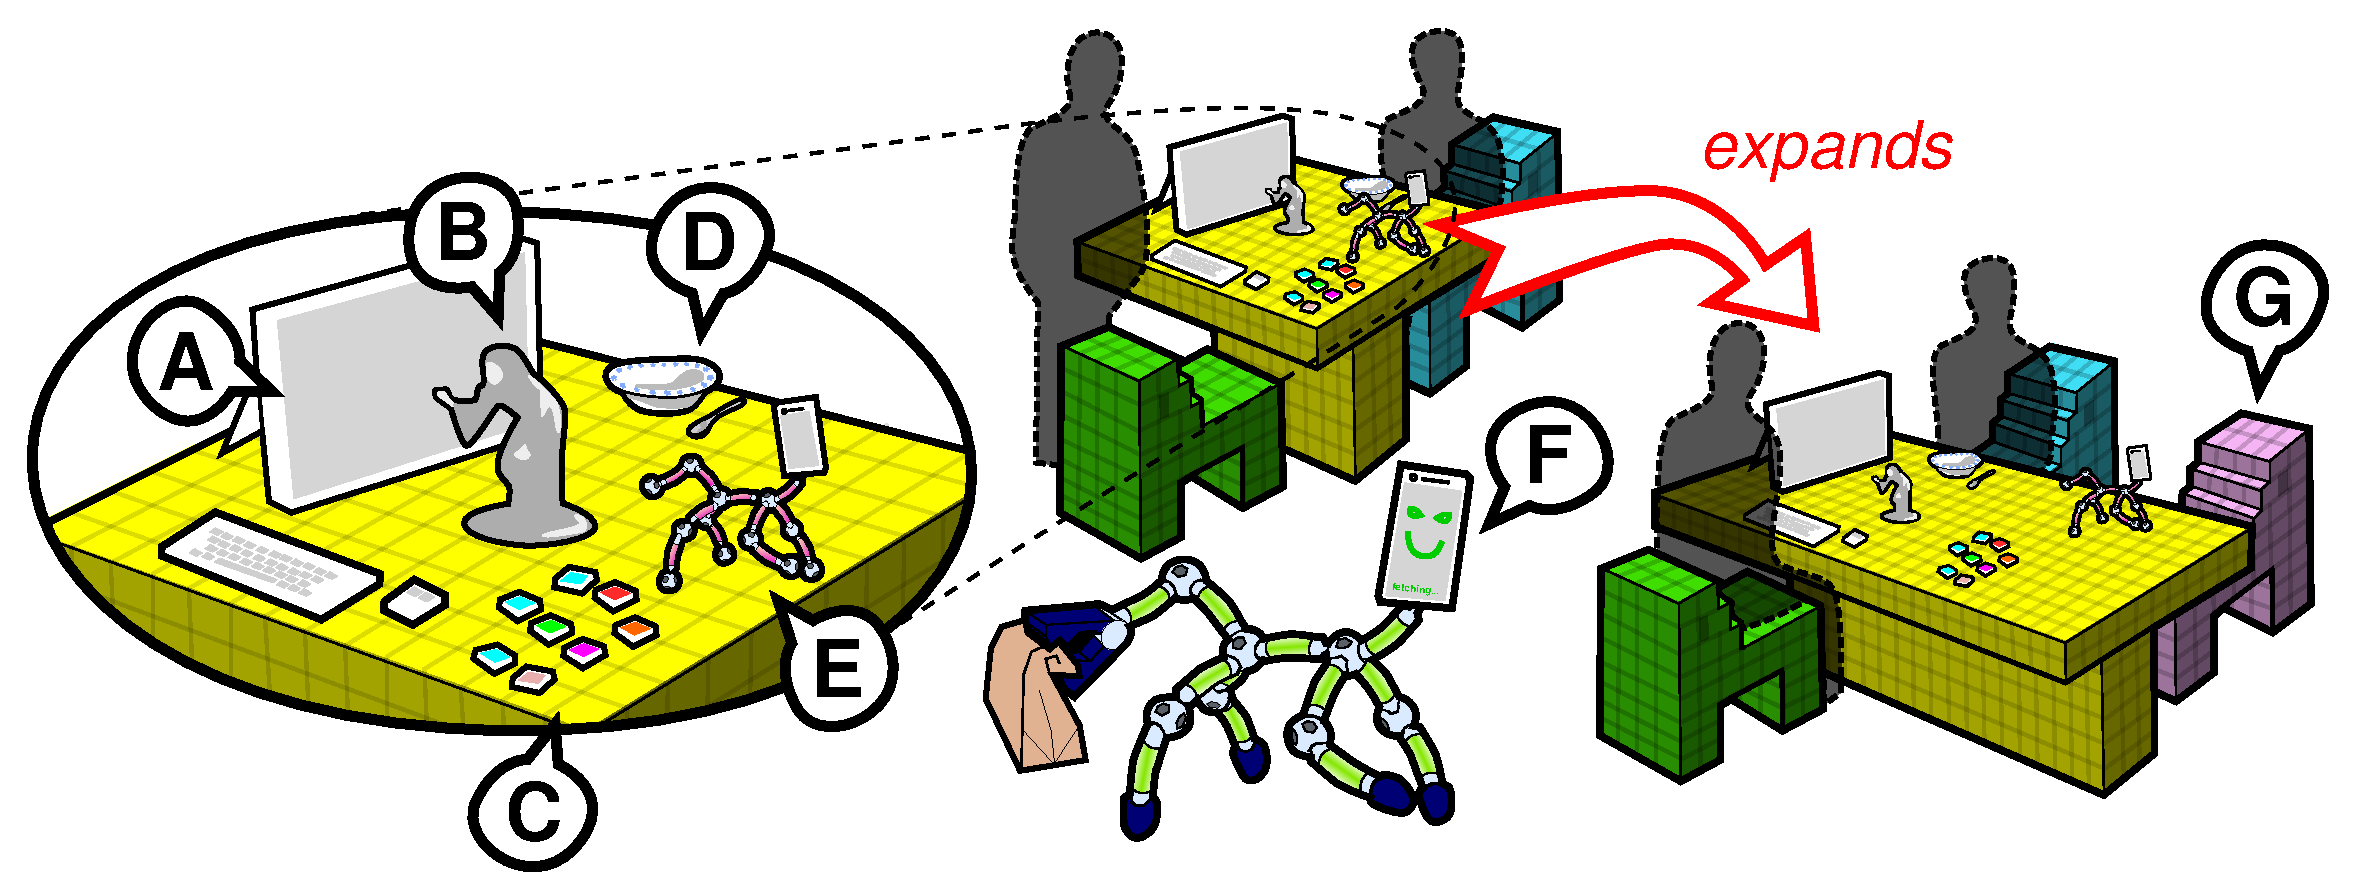
\includegraphics[width=140mm]{kinds_of_artifacts.pdf}
  \caption{An illustration of various kinds of artifacts found in responsive environments: \textbf{\emph{A}} a (work)bench computer (a popsicle); \textbf{\emph{B}} an avatar hyperthou; \textbf{\emph{C}} a tile tinkit; \textbf{\emph{D}} a bowl and spoon (duckcicles); \textbf{\emph{E}} a stickpuppet fig (with a hub-and-strut tinkit body and a volticle crystal for a head); \textbf{\emph{F}} a golem fig fetching lunch; \textbf{\emph{G}} a social table hyperfig (composed of prismatic cube bunkles).}
  \label{fig:kinds_of_artifacts}
\end{figure}

\subsection{Sticks}
%
While many devices in a responsive environment may operate autonomously, it will often be desirable for people to give direct input to control a device. 
We call a device that facilitates realtime control input a `stick', after the classic video game input device the joystick. 

There are several varieties of sticks. 
For example a device that gathers together several buttons and directional controls such as a game controller, or an aerial drone sockpuppet's dedicated control panel, is a \emph{stickboard}. 
The smaller fetchbot model (built with a tinkit) shown in Figure~\ref{fig:kinds_of_artifacts} at \emph{E} could be used as a \emph{stickpuppet} to directly pose the fetchbot golem shown at \emph{F}. 
More nuanced input could be gathered from a partial%
\footnote{For example the g-speak system \citep{gstalt} uses motion capture to identify hand gestures made while wearing special gloves in a space populated with high-resolution video cameras.}
or full-body%
\footnote{For example with a Kinect, an inexpensive system (sold as a peripheral for the XBox video game console) that captures both a depth mapping (using an infrared laser and sensor) and a video stream. This data can be combined to reconstruct a person's full-body pose.}
\emph{sticksuit} that uses either an instrumented space or integrated sensors in clothing (or both) to capture human movement with high fidelity.

\subsection{Shrines}
%
These are systems that provide people with a direct interface to idols or computation.

A crystal is a shrine that supports communication with distant people and idols; a touchscreen with a microphone, one or more cameras, and various sensors and networking interfaces (Figure~\ref{fig:kinds_of_artifacts}, the head of the stickpuppet at \emph{E}). An example is a smartphone or tablet, or to a lesser degree a device such as an ipod touch (as a proper crystal should have an always-on network connection). 

A shrine with expert interfaces (for a tek or tooler) is a \emph{bench} (as in a work bench, shown in Figure~\ref{fig:kinds_of_artifacts} at \emph{A}). A bench often features specialized input devices such as a keyboard, a \textbf{force-feedback pointing device} or a reservoir of bunkles. 

A more powerful collection of computers capable of hosting an idol (such as a server farm) or performing simulations run by a wiz is a \emph{temple}.

\subsection{Badges}
%
While people are adept at visually identifying artifacts and other people, most computational systems need a hint. Badges are devices that can be attached to an artifact or worn by a person to facilitate their identification by responsive devices. Passive badges such as \textbf{QR codes} and \textbf{RFID tags} need to be scanned by a sensor, while active badges such as crystals generally track their own position%
\footnote{Using the \textbf{global positioning system (GPS)} or radio triangulation from known cell towers and wi-fi access points.}
and broadcast it over the network.


\section{Responsive Morphologies}
\label{sec:morphologies}
%
While ducks come in many forms, devices that serve as computational interfaces are generally constrained to one of a few familiar morphologies. The first three (screens, boards and guns) are traditional computational morphologies and the next four are manipulative morphologies (illustrated in Figure~\ref{fig:manipulative_morphologies}) for robunculi.

\subsection{Screens}
%
Many computational interactions revolve around the screen, a display generally composed of individually controllable red, green and blue pixels. Crude screens may only display in two colors (such as black and green) or may only display characters. Some screens also accept input from fingers or styluses.

\subsection{Boards}
%
These devices collect together a variety of buttons, toggles, faders, dials, directional pads, or trackballs to provide a means of giving input to a computer. Some examples are a keyboard, a mouse, a game controller and a music mixing board.

\subsection{Guns}
%
There are many examples of handheld sensors that are operated by pointing them at things: (video) cameras, microphones, laser range finders, thermal sensors. Some of them, such as a target-painting laser, or a surface-to-air missile, can even be used to blow things up. The same devices can often also be mounted on or near a screen (for example a camera) so that they point back at you.

\subsection{Tiles}
%
These manipulatives facilitate arranging tokens in a two-dimensional space. Tiles are useful for describing relationships such as adjacency, grouping and ordering. Due to the simplicity of this morphology they are particularly amenable to having graphics or a screen on their faces. 

\begin{figure}[tbh]
  \centering
    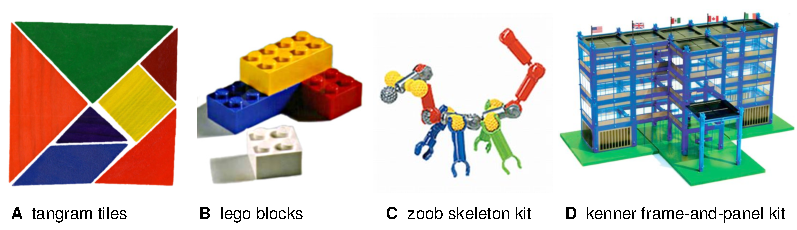
\includegraphics[width=\textwidth]{manipulative_morphologies.pdf}
  \caption{Examples of each of the four manipulative morphologies.}
  \label{fig:manipulative_morphologies}
\end{figure}

\subsection{Blocks}
%
This is the most accessible of the 3D manipulative morphologies, and the most general, as a pile of cubes or lego bricks can be arranged to rasterize almost any 3D form. A limitation of blocks is that achieving a satisfactory level of granularity may require large numbers of modules.

\subsection{Skellies}
%
Named for the skeletons they resemble, this morphology includes hub-and-strut kits (such as tinkertoys), as well as chain link kits (such as zoobs). A skelly can be used to represent abstract graphs or to model articulated forms.

\subsection{Panels}
%
This is a kind of 3D variation of a tile kit. Sometimes panels connect directly to each other to form a load-bearing structure, and sometimes they are attached to a frame.

\section{Responsive Affordances}
\label{sec:affordances}
%
While ducks and manipulatives present various affordances that derive from their forms, responsive artifacts can additionally present affordances that derive from their robotic capabilities. 
These affordances can be organized in input/output pairs, for example our prismatic cubes can sense the fig they have been \emph{placed} in (input), and can self-reconfigure into a new fig on their own (output). 
Below we characterize the six pairs of input/output affordances that a responsive artifact can offer. 
Systems that offer \emph{parallel affordances}---by implementing both the input and output affordances of a pair---benefit from the synergistic effect of being able to repeat what has been demonstrated to them. 
Devices can benefit from a thoughtful combination of manipulative forms and responsive affordances.

\subsection{Placing and Self-reconfiguring}
%
These affordances deal with alterations to the topology of a fig. 
Sytems that afford placing are capable of sensing when a fig's shape is altered by adding, moving or removing bunkles.
Systems that afford self-reconfiguring are capable of rearranging the bunkles of a fig to produce arbitrary forms (within certain constraints). As bunkles capable of self-reconfiguring can be used to realize hyperforms we call these specialized modules \emph{hyperbunkles}.

\subsection{Posing and Flexing}
%
These affordances deal with alterations to a device's pose. 
A system that affords posing is capable of sensing bending, squeezing or stretching a form to alter its shape. 
Systems that afford flexing are capable of actuating these same degrees of freedom to produce arbitrary poses. 
Articulated gaits and wheeled motion are also a form of flexing---reproducing a pattern of poses results in motion through space.

To properly support posing (or flexing) a system must be able to sense (or actuate) all of the mechanical degrees of freedom available in the device. For example the hubs and struts of our Posey kit feature a ball and socket joint that permits three degrees of freedom. By employing a complex sensor to read all three degrees of freedom Posey fully supports posing. Senspectra \cite{senspectra}, another skelly kit, features flexible struts with two degrees of freedom, but only senses the degree of bending and not the direction. It is thus possible (although not necessarily desirable) for a system to only partially support posing (and in a similar manner, flexing).

\subsection{Tapping and Haloing}
%
It is often desirable to pick out one entity among many. Tapping is the input affordance of being able to (perhaps literally) tap on a single entity to indicate it. Haloing is the parallel output affordance of indicating a single entity within a group. These affordances can be presented by bunkles as well as entities rendered on a screen.

These first three pairs of responsive affordances form the basis for tangible interaction as they can be applied synergistically to manipulative morphologies.

\subsection{Tagging and Texting}
%
These affordances refer to the capability to accept text as input---tagging---and to print text as output---texting. They are typically, but not necessarily, implemented with a keyboard and screen, respectively.

These two affordances alone are sufficient to support a \textbf{command line interface}, which is all that many wizzes are looking for in a responsive artifact (provided the interface is coupled to a sufficiently powerful computer and network connection).

\subsection{Graffing and Gramming}
%
Devices that support graffing are capable of accepting drawings as input, either directly with a finger or stylus, or indirectly with a pointing device. Devices that afford gramming have the capability to display graphics (rather than just text).

These affordances, together with tapping and haloing, and tagging and texting, are the basis for the graphical user interfaces which mediate nearly all interaction with shrines (except for command line interfaces, which leverage a subset of the same affordances). By combining text and graphical affordances with tangible affordances, robunculi such as Sifteo tiles support tinkering interfaces to complex systems.

\subsection{Obeying and Mocking}
%
The names of these affordances are intended to evoke behaviors of domesticated animals: dogs are able to obey spoken (and gestural) commands and parrots are capable of mocking (if not necessarily understanding) them. While these affordances may be implemented as an audio interface, it could also involve gestures or other language-like behaviors.

While these audiovisual affordances have not been well supported due to the difficulty of parsing spoken language (not to mention body language), with advances in this technology these interfaces may become more popular. An advantage of an audiovisual interface is that it makes few demands on the morphology of the device and is broadly accessible with little training. These affordances are potentially especially useful for wrangler and taster interaction with golems and ducks, as these devices' morphologies are constrained by their functions.

\section{Devotions}
\label{sec:devotions}
%
While responsive affordances help us to relate to our devices, much of the power of our devices comes from their relationship with idols on the network. 
The structure of this relationship is generally that our devices offer information up to our chosen idols (through the network) and in return they leverage this information to improve search results (through a better understanding of our current context) and manage data that is important to us (among other things%
\footnote{Serving us better is not idols' only motivation for accepting our data; they also use this information to profit their parent organizations through activities such as selling models to marketing agencies.}).
We call these modes that a device can employ to offer up information to an idol \emph{devotions}.

\subsection{Naming} 
%
This devotion allows our devices to vouch for the identity of the bearer. This can be used to identify the source of other devotions; or to give access to resources such as bank accounts at the point of sale;%
\footnote{For example android phones with \textbf{near field communication (NFC)} can use Google Wallet in place of a credit card to pay for things in a store.}
or to give the bearer access to physical spaces by for example opening electronic locks on doors.

\subsection{Slamming} 
%
The name of this devotion is derived from \textbf{simultaneous localization and mapping (SLAM)}, which is the robotic discipline of figuring out where a device is. At its most basic this devotion lets the device communicate to the idol where it is. For example, when you ask an idol for a map on your crystal, it is this devotion that allows the idol to indicate your current position on the map.

More advanced versions of this devotion actually generate maps of areas unknown to an idol (or refine the idol's current maps).

\subsection{Logging} 
%
An advantage of a device with a constant connection to the network is that data can automatically backed up to repositories on the network---devices that automatically mirror their data online practice the devotion of logging. 
An example of a device that supports logging is a crystal; once the naming devotion is initiated with an idol crystals will automatically mirror all contact data so that even if the device is lost your contact information is not. 
And a crystal's camera can be configured to automatically log any photos you take.

By adding custom sensors to crystals, logging has also been used together with slamming to track environmental conditions such as radiation%
\footnote{Safecast, founded in response to government secrecy after the Fukushima reactor meltdown, produces open-hardware radiation sensors that can be plugged into a crystal. Safecast's idol recieves data from devotees and uses it to generate maps of radiation levels.}
and air pollution%
\footnote{For example the researchers for the N-Smarts project gave taxi drivers crystals with bespoke carbon dioxide sensors to generate an air quality map of Accra, Ghana \citep{n-smarts}.}.

\subsection{Tracking} 
%
While slamming allows idols to follow the whereabouts of their devotees, the devotion of tracking consists of devotees identifying and communicating the location of other nearby entities (and possibly other information about the current state of these entities). For example many intersections now feature devices with arrays of cameras that track the cars entering the intersection by reading their license plates. These devices are also tied into the systems operating the traffic signals; anytime a car enters the intersection against the light an additional alert is sent to an idol that issues citations by mail.

\section{Characterizing Responsive Artifacts}
\label{sec:characterizing}
%
The intent of this sketch of responsive artifact ecologies and devices is to allow us to characterize responsive artifacts. By identifying similar systems we can critically examine: their relative effect on the ecology; their relative performance; and opportunities for reuse. To this end we have developed icons (Figure~\ref{fig:icons}) that we will use to summarize the features of responsive artifacts in our survey in Chapter~\ref{ch:survey} and case studies in Chapter~\ref{ch:case_studies}. These icons describe the five categories of features we have introduced above: production, purpose, morphology, affordance and devotion.

\begin{figure}[tbh]
  \centering
    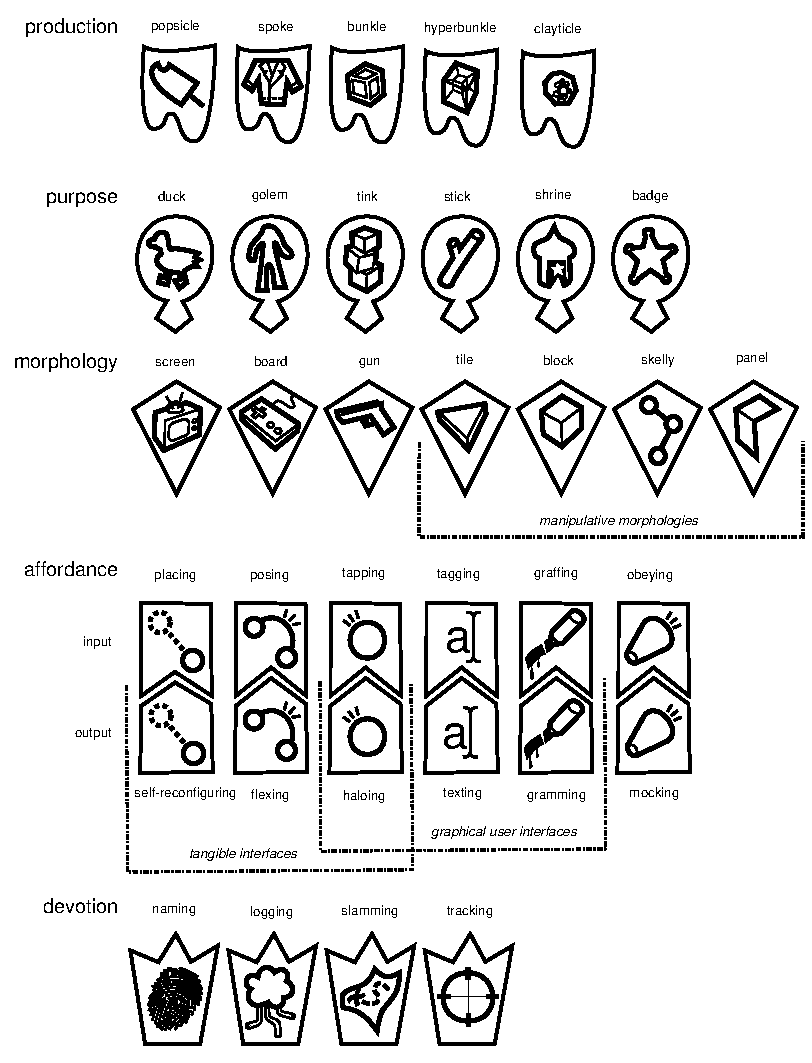
\includegraphics[width=137.5mm]{icons.pdf}
  \caption{Icons representing the characteristics of responsive artifacts.}
  \label{fig:icons}
\end{figure}
